% Created 2018-09-06 Thu 20:53
% Intended LaTeX compiler: pdflatex
\documentclass[11pt]{article}
\usepackage[utf8]{inputenc}
\usepackage[T1]{fontenc}
\usepackage{graphicx}
\usepackage{grffile}
\usepackage{longtable}
\usepackage{wrapfig}
\usepackage{rotating}
\usepackage[normalem]{ulem}
\usepackage{amsmath}
\usepackage{textcomp}
\usepackage{amssymb}
\usepackage{capt-of}
\usepackage{hyperref}
\date{\today}
\title{}
\hypersetup{
 pdfauthor={},
 pdftitle={},
 pdfkeywords={},
 pdfsubject={},
 pdfcreator={Emacs 26.1 (Org mode 9.1.9)}, 
 pdflang={English}}
\begin{document}

\tableofcontents

\section{Wool}
\label{sec:org10dc691}

Wool comes from sheep


\begin{center}
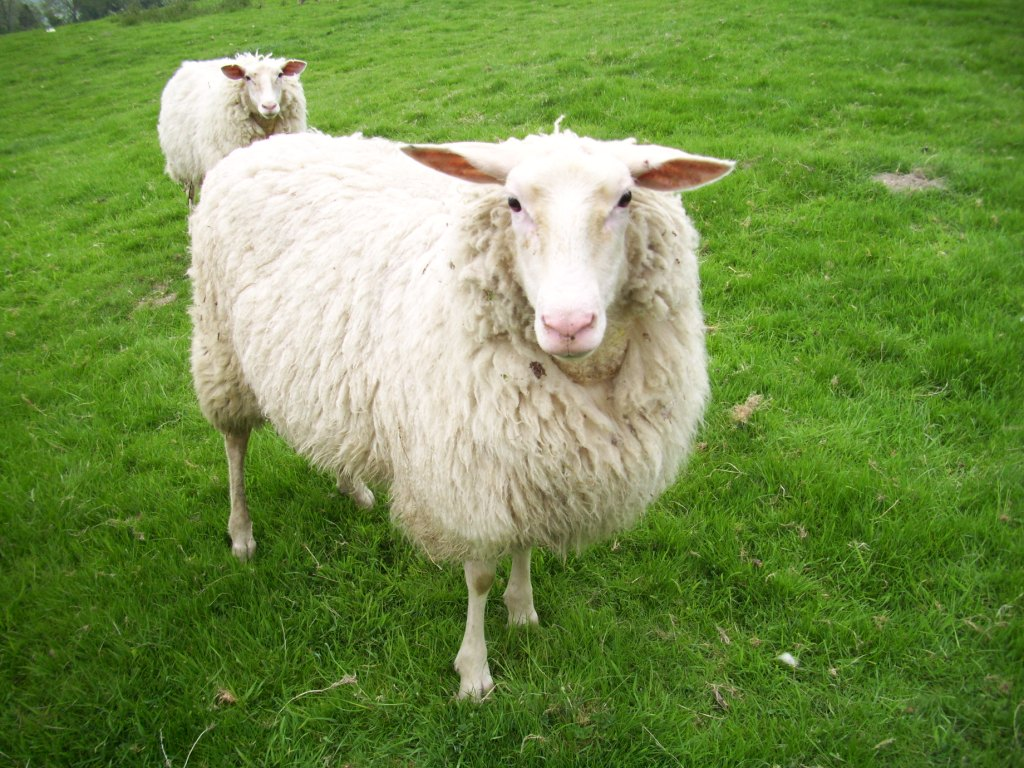
\includegraphics[width=.9\linewidth]{./sheep.jpg}
\end{center}


\subsection{Fabrication}
\label{sec:org33957df}

\subsection{Manufacturing}
\label{sec:org7c49b58}

\subsection{Types of wool}
\label{sec:org5635202}

\subsection{Wool products}
\label{sec:org2f2724d}

\subsection{Environmental impact}
\label{sec:orgf8bd901}
\end{document}
